% Created by tikzDevice version 0.12.3.1 on 2020-08-11 21:12:18
% !TEX encoding = UTF-8 Unicode
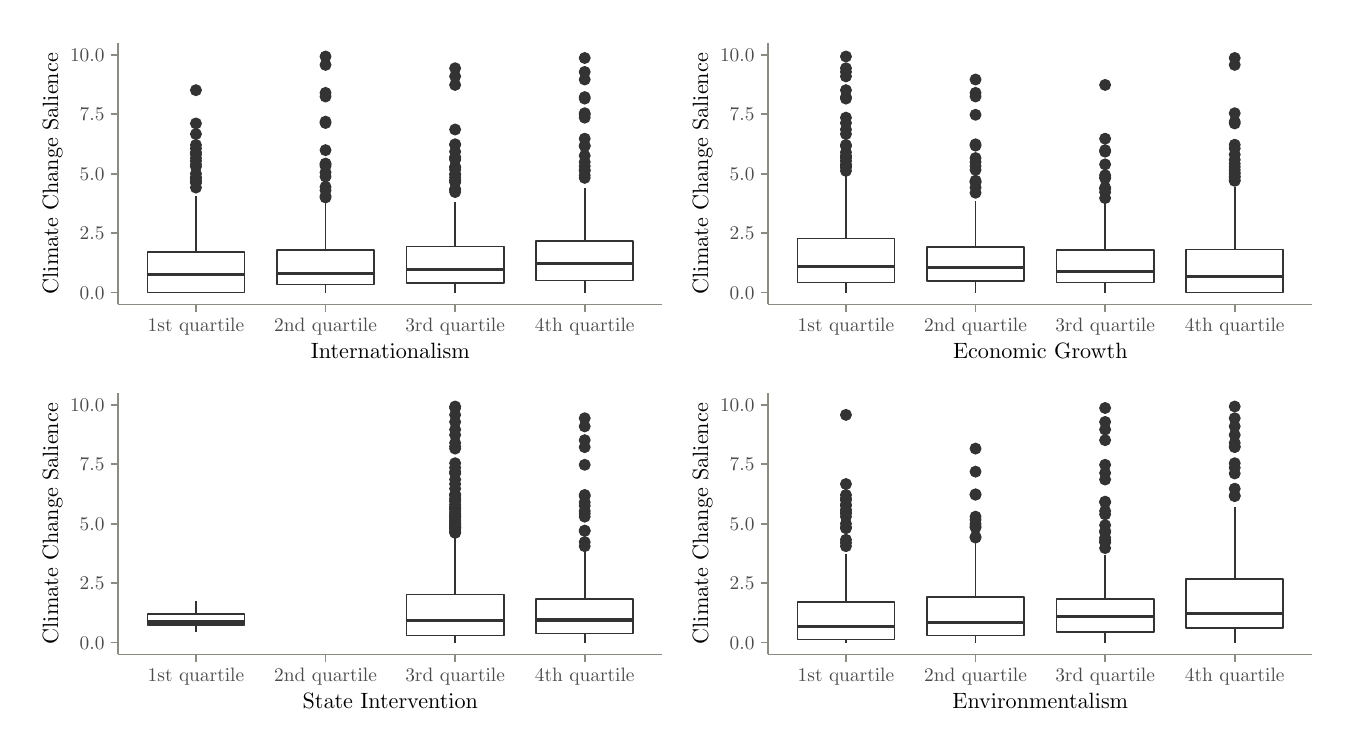
\begin{tikzpicture}[x=1pt,y=1pt]
\definecolor{fillColor}{RGB}{255,255,255}
\path[use as bounding box,fill=fillColor,fill opacity=0.00] (0,0) rectangle (469.76,252.94);
\begin{scope}
\path[clip] ( 32.71,152.92) rectangle (229.38,247.44);
\definecolor{drawColor}{gray}{0.20}
\definecolor{fillColor}{gray}{0.20}

\path[draw=drawColor,line width= 0.4pt,line join=round,line cap=round,fill=fillColor] ( 60.80,197.18) circle (  1.96);

\path[draw=drawColor,line width= 0.4pt,line join=round,line cap=round,fill=fillColor] ( 60.80,214.50) circle (  1.96);

\path[draw=drawColor,line width= 0.4pt,line join=round,line cap=round,fill=fillColor] ( 60.80,209.30) circle (  1.96);

\path[draw=drawColor,line width= 0.4pt,line join=round,line cap=round,fill=fillColor] ( 60.80,195.16) circle (  1.96);

\path[draw=drawColor,line width= 0.4pt,line join=round,line cap=round,fill=fillColor] ( 60.80,200.18) circle (  1.96);

\path[draw=drawColor,line width= 0.4pt,line join=round,line cap=round,fill=fillColor] ( 60.80,197.65) circle (  1.96);

\path[draw=drawColor,line width= 0.4pt,line join=round,line cap=round,fill=fillColor] ( 60.80,218.33) circle (  1.96);

\path[draw=drawColor,line width= 0.4pt,line join=round,line cap=round,fill=fillColor] ( 60.80,196.88) circle (  1.96);

\path[draw=drawColor,line width= 0.4pt,line join=round,line cap=round,fill=fillColor] ( 60.80,198.88) circle (  1.96);

\path[draw=drawColor,line width= 0.4pt,line join=round,line cap=round,fill=fillColor] ( 60.80,230.35) circle (  1.96);

\path[draw=drawColor,line width= 0.4pt,line join=round,line cap=round,fill=fillColor] ( 60.80,204.77) circle (  1.96);

\path[draw=drawColor,line width= 0.4pt,line join=round,line cap=round,fill=fillColor] ( 60.80,202.71) circle (  1.96);

\path[draw=drawColor,line width= 0.4pt,line join=round,line cap=round,fill=fillColor] ( 60.80,205.78) circle (  1.96);

\path[draw=drawColor,line width= 0.4pt,line join=round,line cap=round,fill=fillColor] ( 60.80,203.54) circle (  1.96);

\path[draw=drawColor,line width= 0.4pt,line join=round,line cap=round,fill=fillColor] ( 60.80,198.53) circle (  1.96);

\path[draw=drawColor,line width= 0.4pt,line join=round,line cap=round,fill=fillColor] ( 60.80,207.09) circle (  1.96);

\path[draw=drawColor,line width= 0.4pt,line join=round,line cap=round,fill=fillColor] ( 60.80,210.55) circle (  1.96);

\path[draw=drawColor,line width= 0.4pt,line join=round,line cap=round,fill=fillColor] ( 60.80,207.90) circle (  1.96);

\path[draw=drawColor,line width= 0.6pt,line join=round] ( 60.80,171.97) -- ( 60.80,192.05);

\path[draw=drawColor,line width= 0.6pt,line join=round] ( 60.80,157.22) -- ( 60.80,157.22);
\definecolor{fillColor}{RGB}{255,255,255}

\path[draw=drawColor,line width= 0.6pt,line join=round,line cap=round,fill=fillColor] ( 43.24,171.97) --
	( 43.24,157.22) --
	( 78.36,157.22) --
	( 78.36,171.97) --
	( 43.24,171.97) --
	cycle;

\path[draw=drawColor,line width= 1.1pt,line join=round] ( 43.24,163.73) -- ( 78.36,163.73);
\definecolor{fillColor}{gray}{0.20}

\path[draw=drawColor,line width= 0.4pt,line join=round,line cap=round,fill=fillColor] (107.63,229.37) circle (  1.96);

\path[draw=drawColor,line width= 0.4pt,line join=round,line cap=round,fill=fillColor] (107.63,239.49) circle (  1.96);

\path[draw=drawColor,line width= 0.4pt,line join=round,line cap=round,fill=fillColor] (107.63,228.07) circle (  1.96);

\path[draw=drawColor,line width= 0.4pt,line join=round,line cap=round,fill=fillColor] (107.63,242.52) circle (  1.96);

\path[draw=drawColor,line width= 0.4pt,line join=round,line cap=round,fill=fillColor] (107.63,203.55) circle (  1.96);

\path[draw=drawColor,line width= 0.4pt,line join=round,line cap=round,fill=fillColor] (107.63,195.43) circle (  1.96);

\path[draw=drawColor,line width= 0.4pt,line join=round,line cap=round,fill=fillColor] (107.63,200.62) circle (  1.96);

\path[draw=drawColor,line width= 0.4pt,line join=round,line cap=round,fill=fillColor] (107.63,202.92) circle (  1.96);

\path[draw=drawColor,line width= 0.4pt,line join=round,line cap=round,fill=fillColor] (107.63,194.16) circle (  1.96);

\path[draw=drawColor,line width= 0.4pt,line join=round,line cap=round,fill=fillColor] (107.63,191.59) circle (  1.96);

\path[draw=drawColor,line width= 0.4pt,line join=round,line cap=round,fill=fillColor] (107.63,199.13) circle (  1.96);

\path[draw=drawColor,line width= 0.4pt,line join=round,line cap=round,fill=fillColor] (107.63,218.98) circle (  1.96);

\path[draw=drawColor,line width= 0.4pt,line join=round,line cap=round,fill=fillColor] (107.63,208.68) circle (  1.96);

\path[draw=drawColor,line width= 0.4pt,line join=round,line cap=round,fill=fillColor] (107.63,192.06) circle (  1.96);

\path[draw=drawColor,line width= 0.4pt,line join=round,line cap=round,fill=fillColor] (107.63,203.82) circle (  1.96);

\path[draw=drawColor,line width= 0.4pt,line join=round,line cap=round,fill=fillColor] (107.63,218.49) circle (  1.96);

\path[draw=drawColor,line width= 0.6pt,line join=round] (107.63,172.67) -- (107.63,191.14);

\path[draw=drawColor,line width= 0.6pt,line join=round] (107.63,160.17) -- (107.63,157.22);
\definecolor{fillColor}{RGB}{255,255,255}

\path[draw=drawColor,line width= 0.6pt,line join=round,line cap=round,fill=fillColor] ( 90.07,172.67) --
	( 90.07,160.17) --
	(125.19,160.17) --
	(125.19,172.67) --
	( 90.07,172.67) --
	cycle;

\path[draw=drawColor,line width= 1.1pt,line join=round] ( 90.07,164.15) -- (125.19,164.15);
\definecolor{fillColor}{gray}{0.20}

\path[draw=drawColor,line width= 0.4pt,line join=round,line cap=round,fill=fillColor] (154.46,235.34) circle (  1.96);

\path[draw=drawColor,line width= 0.4pt,line join=round,line cap=round,fill=fillColor] (154.46,205.82) circle (  1.96);

\path[draw=drawColor,line width= 0.4pt,line join=round,line cap=round,fill=fillColor] (154.46,232.25) circle (  1.96);

\path[draw=drawColor,line width= 0.4pt,line join=round,line cap=round,fill=fillColor] (154.46,216.14) circle (  1.96);

\path[draw=drawColor,line width= 0.4pt,line join=round,line cap=round,fill=fillColor] (154.46,194.26) circle (  1.96);

\path[draw=drawColor,line width= 0.4pt,line join=round,line cap=round,fill=fillColor] (154.46,197.86) circle (  1.96);

\path[draw=drawColor,line width= 0.4pt,line join=round,line cap=round,fill=fillColor] (154.46,206.25) circle (  1.96);

\path[draw=drawColor,line width= 0.4pt,line join=round,line cap=round,fill=fillColor] (154.46,238.28) circle (  1.96);

\path[draw=drawColor,line width= 0.4pt,line join=round,line cap=round,fill=fillColor] (154.46,194.67) circle (  1.96);

\path[draw=drawColor,line width= 0.4pt,line join=round,line cap=round,fill=fillColor] (154.46,208.13) circle (  1.96);

\path[draw=drawColor,line width= 0.4pt,line join=round,line cap=round,fill=fillColor] (154.46,199.83) circle (  1.96);

\path[draw=drawColor,line width= 0.4pt,line join=round,line cap=round,fill=fillColor] (154.46,202.44) circle (  1.96);

\path[draw=drawColor,line width= 0.4pt,line join=round,line cap=round,fill=fillColor] (154.46,193.53) circle (  1.96);

\path[draw=drawColor,line width= 0.4pt,line join=round,line cap=round,fill=fillColor] (154.46,210.79) circle (  1.96);

\path[draw=drawColor,line width= 0.4pt,line join=round,line cap=round,fill=fillColor] (154.46,197.60) circle (  1.96);

\path[draw=drawColor,line width= 0.4pt,line join=round,line cap=round,fill=fillColor] (154.46,210.64) circle (  1.96);

\path[draw=drawColor,line width= 0.4pt,line join=round,line cap=round,fill=fillColor] (154.46,198.79) circle (  1.96);

\path[draw=drawColor,line width= 0.4pt,line join=round,line cap=round,fill=fillColor] (154.46,205.20) circle (  1.96);

\path[draw=drawColor,line width= 0.4pt,line join=round,line cap=round,fill=fillColor] (154.46,200.08) circle (  1.96);

\path[draw=drawColor,line width= 0.4pt,line join=round,line cap=round,fill=fillColor] (154.46,201.59) circle (  1.96);

\path[draw=drawColor,line width= 0.4pt,line join=round,line cap=round,fill=fillColor] (154.46,202.71) circle (  1.96);

\path[draw=drawColor,line width= 0.4pt,line join=round,line cap=round,fill=fillColor] (154.46,197.04) circle (  1.96);

\path[draw=drawColor,line width= 0.6pt,line join=round] (154.46,173.84) -- (154.46,189.80);

\path[draw=drawColor,line width= 0.6pt,line join=round] (154.46,160.76) -- (154.46,157.22);
\definecolor{fillColor}{RGB}{255,255,255}

\path[draw=drawColor,line width= 0.6pt,line join=round,line cap=round,fill=fillColor] (136.90,173.84) --
	(136.90,160.76) --
	(172.02,160.76) --
	(172.02,173.84) --
	(136.90,173.84) --
	cycle;

\path[draw=drawColor,line width= 1.1pt,line join=round] (136.90,165.68) -- (172.02,165.68);
\definecolor{fillColor}{gray}{0.20}

\path[draw=drawColor,line width= 0.4pt,line join=round,line cap=round,fill=fillColor] (201.28,234.20) circle (  1.96);

\path[draw=drawColor,line width= 0.4pt,line join=round,line cap=round,fill=fillColor] (201.28,220.42) circle (  1.96);

\path[draw=drawColor,line width= 0.4pt,line join=round,line cap=round,fill=fillColor] (201.28,236.94) circle (  1.96);

\path[draw=drawColor,line width= 0.4pt,line join=round,line cap=round,fill=fillColor] (201.28,198.66) circle (  1.96);

\path[draw=drawColor,line width= 0.4pt,line join=round,line cap=round,fill=fillColor] (201.28,201.20) circle (  1.96);

\path[draw=drawColor,line width= 0.4pt,line join=round,line cap=round,fill=fillColor] (201.28,222.03) circle (  1.96);

\path[draw=drawColor,line width= 0.4pt,line join=round,line cap=round,fill=fillColor] (201.28,210.13) circle (  1.96);

\path[draw=drawColor,line width= 0.4pt,line join=round,line cap=round,fill=fillColor] (201.28,227.31) circle (  1.96);

\path[draw=drawColor,line width= 0.4pt,line join=round,line cap=round,fill=fillColor] (201.28,227.85) circle (  1.96);

\path[draw=drawColor,line width= 0.4pt,line join=round,line cap=round,fill=fillColor] (201.28,206.67) circle (  1.96);

\path[draw=drawColor,line width= 0.4pt,line join=round,line cap=round,fill=fillColor] (201.28,212.82) circle (  1.96);

\path[draw=drawColor,line width= 0.4pt,line join=round,line cap=round,fill=fillColor] (201.28,199.63) circle (  1.96);

\path[draw=drawColor,line width= 0.4pt,line join=round,line cap=round,fill=fillColor] (201.28,241.98) circle (  1.96);

\path[draw=drawColor,line width= 0.4pt,line join=round,line cap=round,fill=fillColor] (201.28,202.88) circle (  1.96);

\path[draw=drawColor,line width= 0.4pt,line join=round,line cap=round,fill=fillColor] (201.28,221.46) circle (  1.96);

\path[draw=drawColor,line width= 0.4pt,line join=round,line cap=round,fill=fillColor] (201.28,204.39) circle (  1.96);

\path[draw=drawColor,line width= 0.4pt,line join=round,line cap=round,fill=fillColor] (201.28,201.55) circle (  1.96);

\path[draw=drawColor,line width= 0.4pt,line join=round,line cap=round,fill=fillColor] (201.28,210.31) circle (  1.96);

\path[draw=drawColor,line width= 0.6pt,line join=round] (201.28,175.84) -- (201.28,195.18);

\path[draw=drawColor,line width= 0.6pt,line join=round] (201.28,161.62) -- (201.28,157.22);
\definecolor{fillColor}{RGB}{255,255,255}

\path[draw=drawColor,line width= 0.6pt,line join=round,line cap=round,fill=fillColor] (183.72,175.84) --
	(183.72,161.62) --
	(218.84,161.62) --
	(218.84,175.84) --
	(183.72,175.84) --
	cycle;

\path[draw=drawColor,line width= 1.1pt,line join=round] (183.72,167.70) -- (218.84,167.70);
\end{scope}
\begin{scope}
\path[clip] (  0.00,  0.00) rectangle (469.76,252.94);
\definecolor{drawColor}{RGB}{139,139,131}

\path[draw=drawColor,line width= 0.6pt,line join=round] ( 32.71,152.92) --
	( 32.71,247.44);
\end{scope}
\begin{scope}
\path[clip] (  0.00,  0.00) rectangle (469.76,252.94);
\definecolor{drawColor}{gray}{0.30}

\node[text=drawColor,anchor=base east,inner sep=0pt, outer sep=0pt, scale=  0.70] at ( 27.76,154.81) {0.0};

\node[text=drawColor,anchor=base east,inner sep=0pt, outer sep=0pt, scale=  0.70] at ( 27.76,176.29) {2.5};

\node[text=drawColor,anchor=base east,inner sep=0pt, outer sep=0pt, scale=  0.70] at ( 27.76,197.77) {5.0};

\node[text=drawColor,anchor=base east,inner sep=0pt, outer sep=0pt, scale=  0.70] at ( 27.76,219.25) {7.5};

\node[text=drawColor,anchor=base east,inner sep=0pt, outer sep=0pt, scale=  0.70] at ( 27.76,240.74) {10.0};
\end{scope}
\begin{scope}
\path[clip] (  0.00,  0.00) rectangle (469.76,252.94);
\definecolor{drawColor}{RGB}{139,139,131}

\path[draw=drawColor,line width= 0.6pt,line join=round] ( 29.96,157.22) --
	( 32.71,157.22);

\path[draw=drawColor,line width= 0.6pt,line join=round] ( 29.96,178.70) --
	( 32.71,178.70);

\path[draw=drawColor,line width= 0.6pt,line join=round] ( 29.96,200.18) --
	( 32.71,200.18);

\path[draw=drawColor,line width= 0.6pt,line join=round] ( 29.96,221.67) --
	( 32.71,221.67);

\path[draw=drawColor,line width= 0.6pt,line join=round] ( 29.96,243.15) --
	( 32.71,243.15);
\end{scope}
\begin{scope}
\path[clip] (  0.00,  0.00) rectangle (469.76,252.94);
\definecolor{drawColor}{RGB}{139,139,131}

\path[draw=drawColor,line width= 0.6pt,line join=round] ( 32.71,152.92) --
	(229.38,152.92);
\end{scope}
\begin{scope}
\path[clip] (  0.00,  0.00) rectangle (469.76,252.94);
\definecolor{drawColor}{RGB}{139,139,131}

\path[draw=drawColor,line width= 0.6pt,line join=round] ( 60.80,150.17) --
	( 60.80,152.92);

\path[draw=drawColor,line width= 0.6pt,line join=round] (107.63,150.17) --
	(107.63,152.92);

\path[draw=drawColor,line width= 0.6pt,line join=round] (154.46,150.17) --
	(154.46,152.92);

\path[draw=drawColor,line width= 0.6pt,line join=round] (201.28,150.17) --
	(201.28,152.92);
\end{scope}
\begin{scope}
\path[clip] (  0.00,  0.00) rectangle (469.76,252.94);
\definecolor{drawColor}{gray}{0.30}

\node[text=drawColor,anchor=base,inner sep=0pt, outer sep=0pt, scale=  0.70] at ( 60.80,143.15) {1st quartile};

\node[text=drawColor,anchor=base,inner sep=0pt, outer sep=0pt, scale=  0.70] at (107.63,143.15) {2nd quartile};

\node[text=drawColor,anchor=base,inner sep=0pt, outer sep=0pt, scale=  0.70] at (154.46,143.15) {3rd quartile};

\node[text=drawColor,anchor=base,inner sep=0pt, outer sep=0pt, scale=  0.70] at (201.28,143.15) {4th quartile};
\end{scope}
\begin{scope}
\path[clip] (  0.00,  0.00) rectangle (469.76,252.94);
\definecolor{drawColor}{RGB}{0,0,0}

\node[text=drawColor,anchor=base,inner sep=0pt, outer sep=0pt, scale=  0.80] at (131.04,133.53) {Internationalism};
\end{scope}
\begin{scope}
\path[clip] (  0.00,  0.00) rectangle (469.76,252.94);
\definecolor{drawColor}{RGB}{0,0,0}

\node[text=drawColor,rotate= 90.00,anchor=base,inner sep=0pt, outer sep=0pt, scale=  0.80] at ( 11.01,200.18) {Climate Change Salience};
\end{scope}
\begin{scope}
\path[clip] (267.58,152.92) rectangle (464.26,247.44);
\definecolor{drawColor}{gray}{0.20}
\definecolor{fillColor}{gray}{0.20}

\path[draw=drawColor,line width= 0.4pt,line join=round,line cap=round,fill=fillColor] (295.68,235.34) circle (  1.96);

\path[draw=drawColor,line width= 0.4pt,line join=round,line cap=round,fill=fillColor] (295.68,216.14) circle (  1.96);

\path[draw=drawColor,line width= 0.4pt,line join=round,line cap=round,fill=fillColor] (295.68,242.52) circle (  1.96);

\path[draw=drawColor,line width= 0.4pt,line join=round,line cap=round,fill=fillColor] (295.68,203.55) circle (  1.96);

\path[draw=drawColor,line width= 0.4pt,line join=round,line cap=round,fill=fillColor] (295.68,214.50) circle (  1.96);

\path[draw=drawColor,line width= 0.4pt,line join=round,line cap=round,fill=fillColor] (295.68,220.42) circle (  1.96);

\path[draw=drawColor,line width= 0.4pt,line join=round,line cap=round,fill=fillColor] (295.68,236.94) circle (  1.96);

\path[draw=drawColor,line width= 0.4pt,line join=round,line cap=round,fill=fillColor] (295.68,201.20) circle (  1.96);

\path[draw=drawColor,line width= 0.4pt,line join=round,line cap=round,fill=fillColor] (295.68,210.13) circle (  1.96);

\path[draw=drawColor,line width= 0.4pt,line join=round,line cap=round,fill=fillColor] (295.68,206.25) circle (  1.96);

\path[draw=drawColor,line width= 0.4pt,line join=round,line cap=round,fill=fillColor] (295.68,238.28) circle (  1.96);

\path[draw=drawColor,line width= 0.4pt,line join=round,line cap=round,fill=fillColor] (295.68,227.31) circle (  1.96);

\path[draw=drawColor,line width= 0.4pt,line join=round,line cap=round,fill=fillColor] (295.68,227.85) circle (  1.96);

\path[draw=drawColor,line width= 0.4pt,line join=round,line cap=round,fill=fillColor] (295.68,206.67) circle (  1.96);

\path[draw=drawColor,line width= 0.4pt,line join=round,line cap=round,fill=fillColor] (295.68,202.92) circle (  1.96);

\path[draw=drawColor,line width= 0.4pt,line join=round,line cap=round,fill=fillColor] (295.68,202.44) circle (  1.96);

\path[draw=drawColor,line width= 0.4pt,line join=round,line cap=round,fill=fillColor] (295.68,230.35) circle (  1.96);

\path[draw=drawColor,line width= 0.4pt,line join=round,line cap=round,fill=fillColor] (295.68,204.77) circle (  1.96);

\path[draw=drawColor,line width= 0.4pt,line join=round,line cap=round,fill=fillColor] (295.68,202.71) circle (  1.96);

\path[draw=drawColor,line width= 0.4pt,line join=round,line cap=round,fill=fillColor] (295.68,205.78) circle (  1.96);

\path[draw=drawColor,line width= 0.4pt,line join=round,line cap=round,fill=fillColor] (295.68,218.49) circle (  1.96);

\path[draw=drawColor,line width= 0.4pt,line join=round,line cap=round,fill=fillColor] (295.68,210.55) circle (  1.96);

\path[draw=drawColor,line width= 0.4pt,line join=round,line cap=round,fill=fillColor] (295.68,207.90) circle (  1.96);

\path[draw=drawColor,line width= 0.6pt,line join=round] (295.68,176.77) -- (295.68,200.18);

\path[draw=drawColor,line width= 0.6pt,line join=round] (295.68,160.83) -- (295.68,157.22);
\definecolor{fillColor}{RGB}{255,255,255}

\path[draw=drawColor,line width= 0.6pt,line join=round,line cap=round,fill=fillColor] (278.12,176.77) --
	(278.12,160.83) --
	(313.24,160.83) --
	(313.24,176.77) --
	(278.12,176.77) --
	cycle;

\path[draw=drawColor,line width= 1.1pt,line join=round] (278.12,166.58) -- (313.24,166.58);
\definecolor{fillColor}{gray}{0.20}

\path[draw=drawColor,line width= 0.4pt,line join=round,line cap=round,fill=fillColor] (342.51,205.82) circle (  1.96);

\path[draw=drawColor,line width= 0.4pt,line join=round,line cap=round,fill=fillColor] (342.51,229.37) circle (  1.96);

\path[draw=drawColor,line width= 0.4pt,line join=round,line cap=round,fill=fillColor] (342.51,234.20) circle (  1.96);

\path[draw=drawColor,line width= 0.4pt,line join=round,line cap=round,fill=fillColor] (342.51,228.07) circle (  1.96);

\path[draw=drawColor,line width= 0.4pt,line join=round,line cap=round,fill=fillColor] (342.51,197.18) circle (  1.96);

\path[draw=drawColor,line width= 0.4pt,line join=round,line cap=round,fill=fillColor] (342.51,195.18) circle (  1.96);

\path[draw=drawColor,line width= 0.4pt,line join=round,line cap=round,fill=fillColor] (342.51,197.65) circle (  1.96);

\path[draw=drawColor,line width= 0.4pt,line join=round,line cap=round,fill=fillColor] (342.51,202.88) circle (  1.96);

\path[draw=drawColor,line width= 0.4pt,line join=round,line cap=round,fill=fillColor] (342.51,221.46) circle (  1.96);

\path[draw=drawColor,line width= 0.4pt,line join=round,line cap=round,fill=fillColor] (342.51,204.39) circle (  1.96);

\path[draw=drawColor,line width= 0.4pt,line join=round,line cap=round,fill=fillColor] (342.51,193.28) circle (  1.96);

\path[draw=drawColor,line width= 0.4pt,line join=round,line cap=round,fill=fillColor] (342.51,201.55) circle (  1.96);

\path[draw=drawColor,line width= 0.4pt,line join=round,line cap=round,fill=fillColor] (342.51,210.31) circle (  1.96);

\path[draw=drawColor,line width= 0.4pt,line join=round,line cap=round,fill=fillColor] (342.51,210.79) circle (  1.96);

\path[draw=drawColor,line width= 0.4pt,line join=round,line cap=round,fill=fillColor] (342.51,197.04) circle (  1.96);

\path[draw=drawColor,line width= 0.6pt,line join=round] (342.51,173.64) -- (342.51,190.23);

\path[draw=drawColor,line width= 0.6pt,line join=round] (342.51,161.36) -- (342.51,157.22);
\definecolor{fillColor}{RGB}{255,255,255}

\path[draw=drawColor,line width= 0.6pt,line join=round,line cap=round,fill=fillColor] (324.95,173.64) --
	(324.95,161.36) --
	(360.07,161.36) --
	(360.07,173.64) --
	(324.95,173.64) --
	cycle;

\path[draw=drawColor,line width= 1.1pt,line join=round] (324.95,166.17) -- (360.07,166.17);
\definecolor{fillColor}{gray}{0.20}

\path[draw=drawColor,line width= 0.4pt,line join=round,line cap=round,fill=fillColor] (389.33,232.25) circle (  1.96);

\path[draw=drawColor,line width= 0.4pt,line join=round,line cap=round,fill=fillColor] (389.33,212.82) circle (  1.96);

\path[draw=drawColor,line width= 0.4pt,line join=round,line cap=round,fill=fillColor] (389.33,199.63) circle (  1.96);

\path[draw=drawColor,line width= 0.4pt,line join=round,line cap=round,fill=fillColor] (389.33,194.67) circle (  1.96);

\path[draw=drawColor,line width= 0.4pt,line join=round,line cap=round,fill=fillColor] (389.33,195.16) circle (  1.96);

\path[draw=drawColor,line width= 0.4pt,line join=round,line cap=round,fill=fillColor] (389.33,191.36) circle (  1.96);

\path[draw=drawColor,line width= 0.4pt,line join=round,line cap=round,fill=fillColor] (389.33,208.13) circle (  1.96);

\path[draw=drawColor,line width= 0.4pt,line join=round,line cap=round,fill=fillColor] (389.33,193.48) circle (  1.96);

\path[draw=drawColor,line width= 0.4pt,line join=round,line cap=round,fill=fillColor] (389.33,208.68) circle (  1.96);

\path[draw=drawColor,line width= 0.4pt,line join=round,line cap=round,fill=fillColor] (389.33,198.79) circle (  1.96);

\path[draw=drawColor,line width= 0.4pt,line join=round,line cap=round,fill=fillColor] (389.33,203.54) circle (  1.96);

\path[draw=drawColor,line width= 0.4pt,line join=round,line cap=round,fill=fillColor] (389.33,198.53) circle (  1.96);

\path[draw=drawColor,line width= 0.6pt,line join=round] (389.33,172.69) -- (389.33,190.14);

\path[draw=drawColor,line width= 0.6pt,line join=round] (389.33,160.88) -- (389.33,157.22);
\definecolor{fillColor}{RGB}{255,255,255}

\path[draw=drawColor,line width= 0.6pt,line join=round,line cap=round,fill=fillColor] (371.77,172.69) --
	(371.77,160.88) --
	(406.89,160.88) --
	(406.89,172.69) --
	(371.77,172.69) --
	cycle;

\path[draw=drawColor,line width= 1.1pt,line join=round] (371.77,164.94) -- (406.89,164.94);
\definecolor{fillColor}{gray}{0.20}

\path[draw=drawColor,line width= 0.4pt,line join=round,line cap=round,fill=fillColor] (436.16,239.49) circle (  1.96);

\path[draw=drawColor,line width= 0.4pt,line join=round,line cap=round,fill=fillColor] (436.16,222.03) circle (  1.96);

\path[draw=drawColor,line width= 0.4pt,line join=round,line cap=round,fill=fillColor] (436.16,197.86) circle (  1.96);

\path[draw=drawColor,line width= 0.4pt,line join=round,line cap=round,fill=fillColor] (436.16,200.62) circle (  1.96);

\path[draw=drawColor,line width= 0.4pt,line join=round,line cap=round,fill=fillColor] (436.16,209.30) circle (  1.96);

\path[draw=drawColor,line width= 0.4pt,line join=round,line cap=round,fill=fillColor] (436.16,241.98) circle (  1.96);

\path[draw=drawColor,line width= 0.4pt,line join=round,line cap=round,fill=fillColor] (436.16,218.33) circle (  1.96);

\path[draw=drawColor,line width= 0.4pt,line join=round,line cap=round,fill=fillColor] (436.16,198.88) circle (  1.96);

\path[draw=drawColor,line width= 0.4pt,line join=round,line cap=round,fill=fillColor] (436.16,199.13) circle (  1.96);

\path[draw=drawColor,line width= 0.4pt,line join=round,line cap=round,fill=fillColor] (436.16,218.98) circle (  1.96);

\path[draw=drawColor,line width= 0.4pt,line join=round,line cap=round,fill=fillColor] (436.16,197.60) circle (  1.96);

\path[draw=drawColor,line width= 0.4pt,line join=round,line cap=round,fill=fillColor] (436.16,210.64) circle (  1.96);

\path[draw=drawColor,line width= 0.4pt,line join=round,line cap=round,fill=fillColor] (436.16,205.20) circle (  1.96);

\path[draw=drawColor,line width= 0.4pt,line join=round,line cap=round,fill=fillColor] (436.16,200.08) circle (  1.96);

\path[draw=drawColor,line width= 0.4pt,line join=round,line cap=round,fill=fillColor] (436.16,201.59) circle (  1.96);

\path[draw=drawColor,line width= 0.4pt,line join=round,line cap=round,fill=fillColor] (436.16,203.82) circle (  1.96);

\path[draw=drawColor,line width= 0.4pt,line join=round,line cap=round,fill=fillColor] (436.16,202.71) circle (  1.96);

\path[draw=drawColor,line width= 0.4pt,line join=round,line cap=round,fill=fillColor] (436.16,207.09) circle (  1.96);

\path[draw=drawColor,line width= 0.6pt,line join=round] (436.16,172.73) -- (436.16,195.43);

\path[draw=drawColor,line width= 0.6pt,line join=round] (436.16,157.22) -- (436.16,157.22);
\definecolor{fillColor}{RGB}{255,255,255}

\path[draw=drawColor,line width= 0.6pt,line join=round,line cap=round,fill=fillColor] (418.60,172.73) --
	(418.60,157.22) --
	(453.72,157.22) --
	(453.72,172.73) --
	(418.60,172.73) --
	cycle;

\path[draw=drawColor,line width= 1.1pt,line join=round] (418.60,163.17) -- (453.72,163.17);
\end{scope}
\begin{scope}
\path[clip] (  0.00,  0.00) rectangle (469.76,252.94);
\definecolor{drawColor}{RGB}{139,139,131}

\path[draw=drawColor,line width= 0.6pt,line join=round] (267.58,152.92) --
	(267.58,247.44);
\end{scope}
\begin{scope}
\path[clip] (  0.00,  0.00) rectangle (469.76,252.94);
\definecolor{drawColor}{gray}{0.30}

\node[text=drawColor,anchor=base east,inner sep=0pt, outer sep=0pt, scale=  0.70] at (262.63,154.81) {0.0};

\node[text=drawColor,anchor=base east,inner sep=0pt, outer sep=0pt, scale=  0.70] at (262.63,176.29) {2.5};

\node[text=drawColor,anchor=base east,inner sep=0pt, outer sep=0pt, scale=  0.70] at (262.63,197.77) {5.0};

\node[text=drawColor,anchor=base east,inner sep=0pt, outer sep=0pt, scale=  0.70] at (262.63,219.25) {7.5};

\node[text=drawColor,anchor=base east,inner sep=0pt, outer sep=0pt, scale=  0.70] at (262.63,240.74) {10.0};
\end{scope}
\begin{scope}
\path[clip] (  0.00,  0.00) rectangle (469.76,252.94);
\definecolor{drawColor}{RGB}{139,139,131}

\path[draw=drawColor,line width= 0.6pt,line join=round] (264.83,157.22) --
	(267.58,157.22);

\path[draw=drawColor,line width= 0.6pt,line join=round] (264.83,178.70) --
	(267.58,178.70);

\path[draw=drawColor,line width= 0.6pt,line join=round] (264.83,200.18) --
	(267.58,200.18);

\path[draw=drawColor,line width= 0.6pt,line join=round] (264.83,221.67) --
	(267.58,221.67);

\path[draw=drawColor,line width= 0.6pt,line join=round] (264.83,243.15) --
	(267.58,243.15);
\end{scope}
\begin{scope}
\path[clip] (  0.00,  0.00) rectangle (469.76,252.94);
\definecolor{drawColor}{RGB}{139,139,131}

\path[draw=drawColor,line width= 0.6pt,line join=round] (267.58,152.92) --
	(464.26,152.92);
\end{scope}
\begin{scope}
\path[clip] (  0.00,  0.00) rectangle (469.76,252.94);
\definecolor{drawColor}{RGB}{139,139,131}

\path[draw=drawColor,line width= 0.6pt,line join=round] (295.68,150.17) --
	(295.68,152.92);

\path[draw=drawColor,line width= 0.6pt,line join=round] (342.51,150.17) --
	(342.51,152.92);

\path[draw=drawColor,line width= 0.6pt,line join=round] (389.33,150.17) --
	(389.33,152.92);

\path[draw=drawColor,line width= 0.6pt,line join=round] (436.16,150.17) --
	(436.16,152.92);
\end{scope}
\begin{scope}
\path[clip] (  0.00,  0.00) rectangle (469.76,252.94);
\definecolor{drawColor}{gray}{0.30}

\node[text=drawColor,anchor=base,inner sep=0pt, outer sep=0pt, scale=  0.70] at (295.68,143.15) {1st quartile};

\node[text=drawColor,anchor=base,inner sep=0pt, outer sep=0pt, scale=  0.70] at (342.51,143.15) {2nd quartile};

\node[text=drawColor,anchor=base,inner sep=0pt, outer sep=0pt, scale=  0.70] at (389.33,143.15) {3rd quartile};

\node[text=drawColor,anchor=base,inner sep=0pt, outer sep=0pt, scale=  0.70] at (436.16,143.15) {4th quartile};
\end{scope}
\begin{scope}
\path[clip] (  0.00,  0.00) rectangle (469.76,252.94);
\definecolor{drawColor}{RGB}{0,0,0}

\node[text=drawColor,anchor=base,inner sep=0pt, outer sep=0pt, scale=  0.80] at (365.92,133.53) {Economic Growth};
\end{scope}
\begin{scope}
\path[clip] (  0.00,  0.00) rectangle (469.76,252.94);
\definecolor{drawColor}{RGB}{0,0,0}

\node[text=drawColor,rotate= 90.00,anchor=base,inner sep=0pt, outer sep=0pt, scale=  0.80] at (245.89,200.18) {Climate Change Salience};
\end{scope}
\begin{scope}
\path[clip] ( 32.71, 26.45) rectangle (229.38,120.97);
\definecolor{drawColor}{gray}{0.20}

\path[draw=drawColor,line width= 0.6pt,line join=round] ( 60.80, 40.98) -- ( 60.80, 45.62);

\path[draw=drawColor,line width= 0.6pt,line join=round] ( 60.80, 37.10) -- ( 60.80, 34.39);
\definecolor{fillColor}{RGB}{255,255,255}

\path[draw=drawColor,line width= 0.6pt,line join=round,line cap=round,fill=fillColor] ( 43.24, 40.98) --
	( 43.24, 37.10) --
	( 78.36, 37.10) --
	( 78.36, 40.98) --
	( 43.24, 40.98) --
	cycle;

\path[draw=drawColor,line width= 1.1pt,line join=round] ( 43.24, 38.18) -- ( 78.36, 38.18);
\definecolor{fillColor}{gray}{0.20}

\path[draw=drawColor,line width= 0.4pt,line join=round,line cap=round,fill=fillColor] (154.46, 79.34) circle (  1.96);

\path[draw=drawColor,line width= 0.4pt,line join=round,line cap=round,fill=fillColor] (154.46,102.90) circle (  1.96);

\path[draw=drawColor,line width= 0.4pt,line join=round,line cap=round,fill=fillColor] (154.46,113.02) circle (  1.96);

\path[draw=drawColor,line width= 0.4pt,line join=round,line cap=round,fill=fillColor] (154.46,105.78) circle (  1.96);

\path[draw=drawColor,line width= 0.4pt,line join=round,line cap=round,fill=fillColor] (154.46,107.72) circle (  1.96);

\path[draw=drawColor,line width= 0.4pt,line join=round,line cap=round,fill=fillColor] (154.46,101.60) circle (  1.96);

\path[draw=drawColor,line width= 0.4pt,line join=round,line cap=round,fill=fillColor] (154.46, 89.66) circle (  1.96);

\path[draw=drawColor,line width= 0.4pt,line join=round,line cap=round,fill=fillColor] (154.46,116.04) circle (  1.96);

\path[draw=drawColor,line width= 0.4pt,line join=round,line cap=round,fill=fillColor] (154.46, 77.08) circle (  1.96);

\path[draw=drawColor,line width= 0.4pt,line join=round,line cap=round,fill=fillColor] (154.46, 70.71) circle (  1.96);

\path[draw=drawColor,line width= 0.4pt,line join=round,line cap=round,fill=fillColor] (154.46, 88.03) circle (  1.96);

\path[draw=drawColor,line width= 0.4pt,line join=round,line cap=round,fill=fillColor] (154.46, 93.94) circle (  1.96);

\path[draw=drawColor,line width= 0.4pt,line join=round,line cap=round,fill=fillColor] (154.46,110.47) circle (  1.96);

\path[draw=drawColor,line width= 0.4pt,line join=round,line cap=round,fill=fillColor] (154.46, 72.19) circle (  1.96);

\path[draw=drawColor,line width= 0.4pt,line join=round,line cap=round,fill=fillColor] (154.46, 74.73) circle (  1.96);

\path[draw=drawColor,line width= 0.4pt,line join=round,line cap=round,fill=fillColor] (154.46, 95.56) circle (  1.96);

\path[draw=drawColor,line width= 0.4pt,line join=round,line cap=round,fill=fillColor] (154.46, 71.39) circle (  1.96);

\path[draw=drawColor,line width= 0.4pt,line join=round,line cap=round,fill=fillColor] (154.46, 79.78) circle (  1.96);

\path[draw=drawColor,line width= 0.4pt,line join=round,line cap=round,fill=fillColor] (154.46,100.84) circle (  1.96);

\path[draw=drawColor,line width= 0.4pt,line join=round,line cap=round,fill=fillColor] (154.46, 74.14) circle (  1.96);

\path[draw=drawColor,line width= 0.4pt,line join=round,line cap=round,fill=fillColor] (154.46, 82.82) circle (  1.96);

\path[draw=drawColor,line width= 0.4pt,line join=round,line cap=round,fill=fillColor] (154.46, 86.35) circle (  1.96);

\path[draw=drawColor,line width= 0.4pt,line join=round,line cap=round,fill=fillColor] (154.46, 73.16) circle (  1.96);

\path[draw=drawColor,line width= 0.4pt,line join=round,line cap=round,fill=fillColor] (154.46,115.51) circle (  1.96);

\path[draw=drawColor,line width= 0.4pt,line join=round,line cap=round,fill=fillColor] (154.46, 76.45) circle (  1.96);

\path[draw=drawColor,line width= 0.4pt,line join=round,line cap=round,fill=fillColor] (154.46, 73.71) circle (  1.96);

\path[draw=drawColor,line width= 0.4pt,line join=round,line cap=round,fill=fillColor] (154.46, 81.66) circle (  1.96);

\path[draw=drawColor,line width= 0.4pt,line join=round,line cap=round,fill=fillColor] (154.46, 76.41) circle (  1.96);

\path[draw=drawColor,line width= 0.4pt,line join=round,line cap=round,fill=fillColor] (154.46, 77.91) circle (  1.96);

\path[draw=drawColor,line width= 0.4pt,line join=round,line cap=round,fill=fillColor] (154.46, 91.86) circle (  1.96);

\path[draw=drawColor,line width= 0.4pt,line join=round,line cap=round,fill=fillColor] (154.46, 73.35) circle (  1.96);

\path[draw=drawColor,line width= 0.4pt,line join=round,line cap=round,fill=fillColor] (154.46, 75.97) circle (  1.96);

\path[draw=drawColor,line width= 0.4pt,line join=round,line cap=round,fill=fillColor] (154.46, 75.07) circle (  1.96);

\path[draw=drawColor,line width= 0.4pt,line join=round,line cap=round,fill=fillColor] (154.46, 70.40) circle (  1.96);

\path[draw=drawColor,line width= 0.4pt,line join=round,line cap=round,fill=fillColor] (154.46, 72.41) circle (  1.96);

\path[draw=drawColor,line width= 0.4pt,line join=round,line cap=round,fill=fillColor] (154.46, 72.66) circle (  1.96);

\path[draw=drawColor,line width= 0.4pt,line join=round,line cap=round,fill=fillColor] (154.46, 83.84) circle (  1.96);

\path[draw=drawColor,line width= 0.4pt,line join=round,line cap=round,fill=fillColor] (154.46, 84.32) circle (  1.96);

\path[draw=drawColor,line width= 0.4pt,line join=round,line cap=round,fill=fillColor] (154.46, 92.51) circle (  1.96);

\path[draw=drawColor,line width= 0.4pt,line join=round,line cap=round,fill=fillColor] (154.46, 76.23) circle (  1.96);

\path[draw=drawColor,line width= 0.4pt,line join=round,line cap=round,fill=fillColor] (154.46, 82.20) circle (  1.96);

\path[draw=drawColor,line width= 0.4pt,line join=round,line cap=round,fill=fillColor] (154.46, 84.17) circle (  1.96);

\path[draw=drawColor,line width= 0.4pt,line join=round,line cap=round,fill=fillColor] (154.46, 79.31) circle (  1.96);

\path[draw=drawColor,line width= 0.4pt,line join=round,line cap=round,fill=fillColor] (154.46, 72.32) circle (  1.96);

\path[draw=drawColor,line width= 0.4pt,line join=round,line cap=round,fill=fillColor] (154.46, 77.07) circle (  1.96);

\path[draw=drawColor,line width= 0.4pt,line join=round,line cap=round,fill=fillColor] (154.46, 78.73) circle (  1.96);

\path[draw=drawColor,line width= 0.4pt,line join=round,line cap=round,fill=fillColor] (154.46, 73.61) circle (  1.96);

\path[draw=drawColor,line width= 0.4pt,line join=round,line cap=round,fill=fillColor] (154.46, 75.12) circle (  1.96);

\path[draw=drawColor,line width= 0.4pt,line join=round,line cap=round,fill=fillColor] (154.46, 72.06) circle (  1.96);

\path[draw=drawColor,line width= 0.4pt,line join=round,line cap=round,fill=fillColor] (154.46, 80.61) circle (  1.96);

\path[draw=drawColor,line width= 0.4pt,line join=round,line cap=round,fill=fillColor] (154.46, 92.02) circle (  1.96);

\path[draw=drawColor,line width= 0.4pt,line join=round,line cap=round,fill=fillColor] (154.46, 70.57) circle (  1.96);

\path[draw=drawColor,line width= 0.6pt,line join=round] (154.46, 48.06) -- (154.46, 68.96);

\path[draw=drawColor,line width= 0.6pt,line join=round] (154.46, 33.28) -- (154.46, 30.74);
\definecolor{fillColor}{RGB}{255,255,255}

\path[draw=drawColor,line width= 0.6pt,line join=round,line cap=round,fill=fillColor] (136.90, 48.06) --
	(136.90, 33.28) --
	(172.02, 33.28) --
	(172.02, 48.06) --
	(136.90, 48.06) --
	cycle;

\path[draw=drawColor,line width= 1.1pt,line join=round] (136.90, 38.56) -- (172.02, 38.56);
\definecolor{fillColor}{gray}{0.20}

\path[draw=drawColor,line width= 0.4pt,line join=round,line cap=round,fill=fillColor] (201.28,108.86) circle (  1.96);

\path[draw=drawColor,line width= 0.4pt,line join=round,line cap=round,fill=fillColor] (201.28, 83.66) circle (  1.96);

\path[draw=drawColor,line width= 0.4pt,line join=round,line cap=round,fill=fillColor] (201.28,111.81) circle (  1.96);

\path[draw=drawColor,line width= 0.4pt,line join=round,line cap=round,fill=fillColor] (201.28,101.37) circle (  1.96);

\path[draw=drawColor,line width= 0.4pt,line join=round,line cap=round,fill=fillColor] (201.28, 80.20) circle (  1.96);

\path[draw=drawColor,line width= 0.4pt,line join=round,line cap=round,fill=fillColor] (201.28, 71.18) circle (  1.96);

\path[draw=drawColor,line width= 0.4pt,line join=round,line cap=round,fill=fillColor] (201.28, 94.98) circle (  1.96);

\path[draw=drawColor,line width= 0.4pt,line join=round,line cap=round,fill=fillColor] (201.28, 67.05) circle (  1.96);

\path[draw=drawColor,line width= 0.4pt,line join=round,line cap=round,fill=fillColor] (201.28,103.88) circle (  1.96);

\path[draw=drawColor,line width= 0.4pt,line join=round,line cap=round,fill=fillColor] (201.28, 78.29) circle (  1.96);

\path[draw=drawColor,line width= 0.4pt,line join=round,line cap=round,fill=fillColor] (201.28, 71.12) circle (  1.96);

\path[draw=drawColor,line width= 0.4pt,line join=round,line cap=round,fill=fillColor] (201.28, 77.35) circle (  1.96);

\path[draw=drawColor,line width= 0.4pt,line join=round,line cap=round,fill=fillColor] (201.28, 76.24) circle (  1.96);

\path[draw=drawColor,line width= 0.4pt,line join=round,line cap=round,fill=fillColor] (201.28, 65.58) circle (  1.96);

\path[draw=drawColor,line width= 0.4pt,line join=round,line cap=round,fill=fillColor] (201.28, 84.08) circle (  1.96);

\path[draw=drawColor,line width= 0.4pt,line join=round,line cap=round,fill=fillColor] (201.28, 81.43) circle (  1.96);

\path[draw=drawColor,line width= 0.6pt,line join=round] (201.28, 46.42) -- (201.28, 63.76);

\path[draw=drawColor,line width= 0.6pt,line join=round] (201.28, 34.04) -- (201.28, 30.74);
\definecolor{fillColor}{RGB}{255,255,255}

\path[draw=drawColor,line width= 0.6pt,line join=round,line cap=round,fill=fillColor] (183.72, 46.42) --
	(183.72, 34.04) --
	(218.84, 34.04) --
	(218.84, 46.42) --
	(183.72, 46.42) --
	cycle;

\path[draw=drawColor,line width= 1.1pt,line join=round] (183.72, 38.90) -- (218.84, 38.90);
\end{scope}
\begin{scope}
\path[clip] (  0.00,  0.00) rectangle (469.76,252.94);
\definecolor{drawColor}{RGB}{139,139,131}

\path[draw=drawColor,line width= 0.6pt,line join=round] ( 32.71, 26.45) --
	( 32.71,120.97);
\end{scope}
\begin{scope}
\path[clip] (  0.00,  0.00) rectangle (469.76,252.94);
\definecolor{drawColor}{gray}{0.30}

\node[text=drawColor,anchor=base east,inner sep=0pt, outer sep=0pt, scale=  0.70] at ( 27.76, 28.33) {0.0};

\node[text=drawColor,anchor=base east,inner sep=0pt, outer sep=0pt, scale=  0.70] at ( 27.76, 49.82) {2.5};

\node[text=drawColor,anchor=base east,inner sep=0pt, outer sep=0pt, scale=  0.70] at ( 27.76, 71.30) {5.0};

\node[text=drawColor,anchor=base east,inner sep=0pt, outer sep=0pt, scale=  0.70] at ( 27.76, 92.78) {7.5};

\node[text=drawColor,anchor=base east,inner sep=0pt, outer sep=0pt, scale=  0.70] at ( 27.76,114.27) {10.0};
\end{scope}
\begin{scope}
\path[clip] (  0.00,  0.00) rectangle (469.76,252.94);
\definecolor{drawColor}{RGB}{139,139,131}

\path[draw=drawColor,line width= 0.6pt,line join=round] ( 29.96, 30.74) --
	( 32.71, 30.74);

\path[draw=drawColor,line width= 0.6pt,line join=round] ( 29.96, 52.23) --
	( 32.71, 52.23);

\path[draw=drawColor,line width= 0.6pt,line join=round] ( 29.96, 73.71) --
	( 32.71, 73.71);

\path[draw=drawColor,line width= 0.6pt,line join=round] ( 29.96, 95.19) --
	( 32.71, 95.19);

\path[draw=drawColor,line width= 0.6pt,line join=round] ( 29.96,116.68) --
	( 32.71,116.68);
\end{scope}
\begin{scope}
\path[clip] (  0.00,  0.00) rectangle (469.76,252.94);
\definecolor{drawColor}{RGB}{139,139,131}

\path[draw=drawColor,line width= 0.6pt,line join=round] ( 32.71, 26.45) --
	(229.38, 26.45);
\end{scope}
\begin{scope}
\path[clip] (  0.00,  0.00) rectangle (469.76,252.94);
\definecolor{drawColor}{RGB}{139,139,131}

\path[draw=drawColor,line width= 0.6pt,line join=round] ( 60.80, 23.70) --
	( 60.80, 26.45);

\path[draw=drawColor,line width= 0.6pt,line join=round] (107.63, 23.70) --
	(107.63, 26.45);

\path[draw=drawColor,line width= 0.6pt,line join=round] (154.46, 23.70) --
	(154.46, 26.45);

\path[draw=drawColor,line width= 0.6pt,line join=round] (201.28, 23.70) --
	(201.28, 26.45);
\end{scope}
\begin{scope}
\path[clip] (  0.00,  0.00) rectangle (469.76,252.94);
\definecolor{drawColor}{gray}{0.30}

\node[text=drawColor,anchor=base,inner sep=0pt, outer sep=0pt, scale=  0.70] at ( 60.80, 16.68) {1st quartile};

\node[text=drawColor,anchor=base,inner sep=0pt, outer sep=0pt, scale=  0.70] at (107.63, 16.68) {2nd quartile};

\node[text=drawColor,anchor=base,inner sep=0pt, outer sep=0pt, scale=  0.70] at (154.46, 16.68) {3rd quartile};

\node[text=drawColor,anchor=base,inner sep=0pt, outer sep=0pt, scale=  0.70] at (201.28, 16.68) {4th quartile};
\end{scope}
\begin{scope}
\path[clip] (  0.00,  0.00) rectangle (469.76,252.94);
\definecolor{drawColor}{RGB}{0,0,0}

\node[text=drawColor,anchor=base,inner sep=0pt, outer sep=0pt, scale=  0.80] at (131.04,  7.06) {State Intervention};
\end{scope}
\begin{scope}
\path[clip] (  0.00,  0.00) rectangle (469.76,252.94);
\definecolor{drawColor}{RGB}{0,0,0}

\node[text=drawColor,rotate= 90.00,anchor=base,inner sep=0pt, outer sep=0pt, scale=  0.80] at ( 11.01, 73.71) {Climate Change Salience};
\end{scope}
\begin{scope}
\path[clip] (267.58, 26.45) rectangle (464.26,120.97);
\definecolor{drawColor}{gray}{0.20}
\definecolor{fillColor}{gray}{0.20}

\path[draw=drawColor,line width= 0.4pt,line join=round,line cap=round,fill=fillColor] (295.68,113.02) circle (  1.96);

\path[draw=drawColor,line width= 0.4pt,line join=round,line cap=round,fill=fillColor] (295.68, 88.03) circle (  1.96);

\path[draw=drawColor,line width= 0.4pt,line join=round,line cap=round,fill=fillColor] (295.68, 80.20) circle (  1.96);

\path[draw=drawColor,line width= 0.4pt,line join=round,line cap=round,fill=fillColor] (295.68, 82.82) circle (  1.96);

\path[draw=drawColor,line width= 0.4pt,line join=round,line cap=round,fill=fillColor] (295.68, 73.71) circle (  1.96);

\path[draw=drawColor,line width= 0.4pt,line join=round,line cap=round,fill=fillColor] (295.68, 77.91) circle (  1.96);

\path[draw=drawColor,line width= 0.4pt,line join=round,line cap=round,fill=fillColor] (295.68, 66.81) circle (  1.96);

\path[draw=drawColor,line width= 0.4pt,line join=round,line cap=round,fill=fillColor] (295.68, 72.41) circle (  1.96);

\path[draw=drawColor,line width= 0.4pt,line join=round,line cap=round,fill=fillColor] (295.68, 76.23) circle (  1.96);

\path[draw=drawColor,line width= 0.4pt,line join=round,line cap=round,fill=fillColor] (295.68, 82.20) circle (  1.96);

\path[draw=drawColor,line width= 0.4pt,line join=round,line cap=round,fill=fillColor] (295.68, 67.89) circle (  1.96);

\path[draw=drawColor,line width= 0.4pt,line join=round,line cap=round,fill=fillColor] (295.68, 78.73) circle (  1.96);

\path[draw=drawColor,line width= 0.4pt,line join=round,line cap=round,fill=fillColor] (295.68, 77.35) circle (  1.96);

\path[draw=drawColor,line width= 0.4pt,line join=round,line cap=round,fill=fillColor] (295.68, 65.58) circle (  1.96);

\path[draw=drawColor,line width= 0.4pt,line join=round,line cap=round,fill=fillColor] (295.68, 72.06) circle (  1.96);

\path[draw=drawColor,line width= 0.4pt,line join=round,line cap=round,fill=fillColor] (295.68, 80.61) circle (  1.96);

\path[draw=drawColor,line width= 0.4pt,line join=round,line cap=round,fill=fillColor] (295.68, 84.08) circle (  1.96);

\path[draw=drawColor,line width= 0.6pt,line join=round] (295.68, 45.31) -- (295.68, 62.57);

\path[draw=drawColor,line width= 0.6pt,line join=round] (295.68, 31.88) -- (295.68, 30.74);
\definecolor{fillColor}{RGB}{255,255,255}

\path[draw=drawColor,line width= 0.6pt,line join=round,line cap=round,fill=fillColor] (278.12, 45.31) --
	(278.12, 31.88) --
	(313.24, 31.88) --
	(313.24, 45.31) --
	(278.12, 45.31) --
	cycle;

\path[draw=drawColor,line width= 1.1pt,line join=round] (278.12, 36.49) -- (313.24, 36.49);
\definecolor{fillColor}{gray}{0.20}

\path[draw=drawColor,line width= 0.4pt,line join=round,line cap=round,fill=fillColor] (342.51, 68.96) circle (  1.96);

\path[draw=drawColor,line width= 0.4pt,line join=round,line cap=round,fill=fillColor] (342.51,100.84) circle (  1.96);

\path[draw=drawColor,line width= 0.4pt,line join=round,line cap=round,fill=fillColor] (342.51, 68.68) circle (  1.96);

\path[draw=drawColor,line width= 0.4pt,line join=round,line cap=round,fill=fillColor] (342.51, 72.66) circle (  1.96);

\path[draw=drawColor,line width= 0.4pt,line join=round,line cap=round,fill=fillColor] (342.51, 84.32) circle (  1.96);

\path[draw=drawColor,line width= 0.4pt,line join=round,line cap=round,fill=fillColor] (342.51, 92.51) circle (  1.96);

\path[draw=drawColor,line width= 0.4pt,line join=round,line cap=round,fill=fillColor] (342.51, 84.17) circle (  1.96);

\path[draw=drawColor,line width= 0.4pt,line join=round,line cap=round,fill=fillColor] (342.51, 72.32) circle (  1.96);

\path[draw=drawColor,line width= 0.4pt,line join=round,line cap=round,fill=fillColor] (342.51, 73.61) circle (  1.96);

\path[draw=drawColor,line width= 0.4pt,line join=round,line cap=round,fill=fillColor] (342.51, 75.12) circle (  1.96);

\path[draw=drawColor,line width= 0.4pt,line join=round,line cap=round,fill=fillColor] (342.51, 76.24) circle (  1.96);

\path[draw=drawColor,line width= 0.6pt,line join=round] (342.51, 47.21) -- (342.51, 67.69);

\path[draw=drawColor,line width= 0.6pt,line join=round] (342.51, 33.34) -- (342.51, 30.74);
\definecolor{fillColor}{RGB}{255,255,255}

\path[draw=drawColor,line width= 0.6pt,line join=round,line cap=round,fill=fillColor] (324.95, 47.21) --
	(324.95, 33.34) --
	(360.07, 33.34) --
	(360.07, 47.21) --
	(324.95, 47.21) --
	cycle;

\path[draw=drawColor,line width= 1.1pt,line join=round] (324.95, 37.87) -- (360.07, 37.87);
\definecolor{fillColor}{gray}{0.20}

\path[draw=drawColor,line width= 0.4pt,line join=round,line cap=round,fill=fillColor] (389.33,107.72) circle (  1.96);

\path[draw=drawColor,line width= 0.4pt,line join=round,line cap=round,fill=fillColor] (389.33, 89.66) circle (  1.96);

\path[draw=drawColor,line width= 0.4pt,line join=round,line cap=round,fill=fillColor] (389.33, 77.08) circle (  1.96);

\path[draw=drawColor,line width= 0.4pt,line join=round,line cap=round,fill=fillColor] (389.33, 67.78) circle (  1.96);

\path[draw=drawColor,line width= 0.4pt,line join=round,line cap=round,fill=fillColor] (389.33,110.47) circle (  1.96);

\path[draw=drawColor,line width= 0.4pt,line join=round,line cap=round,fill=fillColor] (389.33, 68.61) circle (  1.96);

\path[draw=drawColor,line width= 0.4pt,line join=round,line cap=round,fill=fillColor] (389.33, 73.16) circle (  1.96);

\path[draw=drawColor,line width= 0.4pt,line join=round,line cap=round,fill=fillColor] (389.33,115.51) circle (  1.96);

\path[draw=drawColor,line width= 0.4pt,line join=round,line cap=round,fill=fillColor] (389.33, 64.89) circle (  1.96);

\path[draw=drawColor,line width= 0.4pt,line join=round,line cap=round,fill=fillColor] (389.33, 81.66) circle (  1.96);

\path[draw=drawColor,line width= 0.4pt,line join=round,line cap=round,fill=fillColor] (389.33, 94.98) circle (  1.96);

\path[draw=drawColor,line width= 0.4pt,line join=round,line cap=round,fill=fillColor] (389.33, 67.05) circle (  1.96);

\path[draw=drawColor,line width= 0.4pt,line join=round,line cap=round,fill=fillColor] (389.33,103.88) circle (  1.96);

\path[draw=drawColor,line width= 0.4pt,line join=round,line cap=round,fill=fillColor] (389.33, 67.01) circle (  1.96);

\path[draw=drawColor,line width= 0.4pt,line join=round,line cap=round,fill=fillColor] (389.33, 78.29) circle (  1.96);

\path[draw=drawColor,line width= 0.4pt,line join=round,line cap=round,fill=fillColor] (389.33, 71.12) circle (  1.96);

\path[draw=drawColor,line width= 0.4pt,line join=round,line cap=round,fill=fillColor] (389.33, 92.02) circle (  1.96);

\path[draw=drawColor,line width= 0.4pt,line join=round,line cap=round,fill=fillColor] (389.33, 70.57) circle (  1.96);

\path[draw=drawColor,line width= 0.4pt,line join=round,line cap=round,fill=fillColor] (389.33, 81.43) circle (  1.96);

\path[draw=drawColor,line width= 0.6pt,line join=round] (389.33, 46.43) -- (389.33, 62.32);

\path[draw=drawColor,line width= 0.6pt,line join=round] (389.33, 34.53) -- (389.33, 30.74);
\definecolor{fillColor}{RGB}{255,255,255}

\path[draw=drawColor,line width= 0.6pt,line join=round,line cap=round,fill=fillColor] (371.77, 46.43) --
	(371.77, 34.53) --
	(406.89, 34.53) --
	(406.89, 46.43) --
	(371.77, 46.43) --
	cycle;

\path[draw=drawColor,line width= 1.1pt,line join=round] (371.77, 40.06) -- (406.89, 40.06);
\definecolor{fillColor}{gray}{0.20}

\path[draw=drawColor,line width= 0.4pt,line join=round,line cap=round,fill=fillColor] (436.16,108.86) circle (  1.96);

\path[draw=drawColor,line width= 0.4pt,line join=round,line cap=round,fill=fillColor] (436.16,102.90) circle (  1.96);

\path[draw=drawColor,line width= 0.4pt,line join=round,line cap=round,fill=fillColor] (436.16,105.78) circle (  1.96);

\path[draw=drawColor,line width= 0.4pt,line join=round,line cap=round,fill=fillColor] (436.16,101.60) circle (  1.96);

\path[draw=drawColor,line width= 0.4pt,line join=round,line cap=round,fill=fillColor] (436.16,116.04) circle (  1.96);

\path[draw=drawColor,line width= 0.4pt,line join=round,line cap=round,fill=fillColor] (436.16, 93.94) circle (  1.96);

\path[draw=drawColor,line width= 0.4pt,line join=round,line cap=round,fill=fillColor] (436.16, 95.56) circle (  1.96);

\path[draw=drawColor,line width= 0.4pt,line join=round,line cap=round,fill=fillColor] (436.16, 83.66) circle (  1.96);

\path[draw=drawColor,line width= 0.4pt,line join=round,line cap=round,fill=fillColor] (436.16,111.81) circle (  1.96);

\path[draw=drawColor,line width= 0.4pt,line join=round,line cap=round,fill=fillColor] (436.16,101.37) circle (  1.96);

\path[draw=drawColor,line width= 0.4pt,line join=round,line cap=round,fill=fillColor] (436.16, 86.35) circle (  1.96);

\path[draw=drawColor,line width= 0.4pt,line join=round,line cap=round,fill=fillColor] (436.16, 91.86) circle (  1.96);

\path[draw=drawColor,line width= 0.4pt,line join=round,line cap=round,fill=fillColor] (436.16, 83.84) circle (  1.96);

\path[draw=drawColor,line width= 0.6pt,line join=round] (436.16, 53.75) -- (436.16, 79.78);

\path[draw=drawColor,line width= 0.6pt,line join=round] (436.16, 36.10) -- (436.16, 30.74);
\definecolor{fillColor}{RGB}{255,255,255}

\path[draw=drawColor,line width= 0.6pt,line join=round,line cap=round,fill=fillColor] (418.60, 53.75) --
	(418.60, 36.10) --
	(453.72, 36.10) --
	(453.72, 53.75) --
	(418.60, 53.75) --
	cycle;

\path[draw=drawColor,line width= 1.1pt,line join=round] (418.60, 41.20) -- (453.72, 41.20);
\end{scope}
\begin{scope}
\path[clip] (  0.00,  0.00) rectangle (469.76,252.94);
\definecolor{drawColor}{RGB}{139,139,131}

\path[draw=drawColor,line width= 0.6pt,line join=round] (267.58, 26.45) --
	(267.58,120.97);
\end{scope}
\begin{scope}
\path[clip] (  0.00,  0.00) rectangle (469.76,252.94);
\definecolor{drawColor}{gray}{0.30}

\node[text=drawColor,anchor=base east,inner sep=0pt, outer sep=0pt, scale=  0.70] at (262.63, 28.33) {0.0};

\node[text=drawColor,anchor=base east,inner sep=0pt, outer sep=0pt, scale=  0.70] at (262.63, 49.82) {2.5};

\node[text=drawColor,anchor=base east,inner sep=0pt, outer sep=0pt, scale=  0.70] at (262.63, 71.30) {5.0};

\node[text=drawColor,anchor=base east,inner sep=0pt, outer sep=0pt, scale=  0.70] at (262.63, 92.78) {7.5};

\node[text=drawColor,anchor=base east,inner sep=0pt, outer sep=0pt, scale=  0.70] at (262.63,114.27) {10.0};
\end{scope}
\begin{scope}
\path[clip] (  0.00,  0.00) rectangle (469.76,252.94);
\definecolor{drawColor}{RGB}{139,139,131}

\path[draw=drawColor,line width= 0.6pt,line join=round] (264.83, 30.74) --
	(267.58, 30.74);

\path[draw=drawColor,line width= 0.6pt,line join=round] (264.83, 52.23) --
	(267.58, 52.23);

\path[draw=drawColor,line width= 0.6pt,line join=round] (264.83, 73.71) --
	(267.58, 73.71);

\path[draw=drawColor,line width= 0.6pt,line join=round] (264.83, 95.19) --
	(267.58, 95.19);

\path[draw=drawColor,line width= 0.6pt,line join=round] (264.83,116.68) --
	(267.58,116.68);
\end{scope}
\begin{scope}
\path[clip] (  0.00,  0.00) rectangle (469.76,252.94);
\definecolor{drawColor}{RGB}{139,139,131}

\path[draw=drawColor,line width= 0.6pt,line join=round] (267.58, 26.45) --
	(464.26, 26.45);
\end{scope}
\begin{scope}
\path[clip] (  0.00,  0.00) rectangle (469.76,252.94);
\definecolor{drawColor}{RGB}{139,139,131}

\path[draw=drawColor,line width= 0.6pt,line join=round] (295.68, 23.70) --
	(295.68, 26.45);

\path[draw=drawColor,line width= 0.6pt,line join=round] (342.51, 23.70) --
	(342.51, 26.45);

\path[draw=drawColor,line width= 0.6pt,line join=round] (389.33, 23.70) --
	(389.33, 26.45);

\path[draw=drawColor,line width= 0.6pt,line join=round] (436.16, 23.70) --
	(436.16, 26.45);
\end{scope}
\begin{scope}
\path[clip] (  0.00,  0.00) rectangle (469.76,252.94);
\definecolor{drawColor}{gray}{0.30}

\node[text=drawColor,anchor=base,inner sep=0pt, outer sep=0pt, scale=  0.70] at (295.68, 16.68) {1st quartile};

\node[text=drawColor,anchor=base,inner sep=0pt, outer sep=0pt, scale=  0.70] at (342.51, 16.68) {2nd quartile};

\node[text=drawColor,anchor=base,inner sep=0pt, outer sep=0pt, scale=  0.70] at (389.33, 16.68) {3rd quartile};

\node[text=drawColor,anchor=base,inner sep=0pt, outer sep=0pt, scale=  0.70] at (436.16, 16.68) {4th quartile};
\end{scope}
\begin{scope}
\path[clip] (  0.00,  0.00) rectangle (469.76,252.94);
\definecolor{drawColor}{RGB}{0,0,0}

\node[text=drawColor,anchor=base,inner sep=0pt, outer sep=0pt, scale=  0.80] at (365.92,  7.06) {Environmentalism};
\end{scope}
\begin{scope}
\path[clip] (  0.00,  0.00) rectangle (469.76,252.94);
\definecolor{drawColor}{RGB}{0,0,0}

\node[text=drawColor,rotate= 90.00,anchor=base,inner sep=0pt, outer sep=0pt, scale=  0.80] at (245.89, 73.71) {Climate Change Salience};
\end{scope}
\end{tikzpicture}
